\section{Image Segmentation}
\subsection{Datasets and Metrics}
1. \textbf{Datasets:} PASCAL VOC, COCO, Cityscapes, etc. \\
   a. Positive: Foreground. \\
   b. Negative: Background. \\
2. \textbf{Metrics:} \\
   a. \[
      \text{Pixel Acc} = \frac{\text{TP} + \text{TN}}{\text{TP} + \text{TN} + \text{FP} + \text{FN}}
      \] \\
   b. 
      \[
      \text{IoU(Jaccard Index)} = \frac{\text{TP}}{\text{TP+FP+FN}}
      \] \\
   c. mIoU (Mean IoU for Multi-Class) \\
   d. F1 Score (DICE): 
      \[
      F1 = 2 \cdot \frac{\text{Precision} \cdot \text{Recall}}{\text{Precision} + \text{Recall}}, 
    \text{DICE} = \frac{2 \cdot \text{Prediction} \cap \text{GT}}{\text{Prediction} + \text{GT}}
    \] 
    \[
    DICE = F1 = \frac{2 \cdot \text{TP}}{2 \cdot \text{TP} + \text{FP} + \text{FN}}
    \]
   Note: DICE same as F1 score in pixel seg.\\
   F score: Closer to avg performance. IoU: Worst-case performance.


\subsection{Approaches to Segmentation}
1. \textbf{Traditional:} Cluster based on color/position. \\
2. \textbf{Sliding Windows:} Inefficient. \\
3. \textbf{End-to-End Fully Conv Network (FCN):}  \\
   a. Downsample\\
   b. Upsample: \\
   i.  Nearest Neighbors \\
   ii. "Bed of nails" \\
   iii. Max unpooling: uses max pos from pooling layers. \\
   iv. Transpose Conv: Learnable. \\
      \[
      L_{\text{out}} = (\text{L}_{\text{in}} - 1) \cdot S + K - 2P
      \] \\
      If pad = 1, the 1st col/row will be removed in the output. \\
      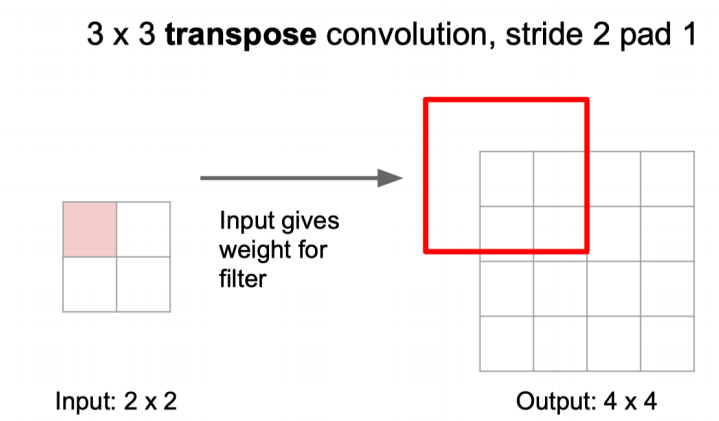
\includegraphics[width=0.8\linewidth]{images/trans-conv.png}

      
4. \textbf{U-Net:}  
      i. Skip connections for low (high res) and high (low res) levels. \\
      ii. Fuse using concatenation.